\chapter{Formula��o Num�rica}
\label{ch:form_num}

% Short comparison FEM and FDM(Papasta)
The basic idea of almost all numerical methods for the solution of PDEs is the discretization and thereby reduction to a finite number of degrees of freedom (DOFs) of a continuum problem, which possesses a infinite number of DOFs. This discrete problem results in an system of equations with finite number of variables, which can normally be solved using an adequate method (see section \ref{sc:multigrid} for details) \citep{Chen2006}.

In the Finite Difference Method (FDM), which is still the standard for numerical reservoir simulations, the derivatives of the original equations are simply replaced by quotients of differences. The values of the variables are defined only in a specified number of points, which can be located either on the corners or in the interior of the cells \citep{Fortuna2000}.

The discretization process within the Finite Element Method (FEM) is different in that it requires a reformulation of the PDEs in an equivalent variational form. The unknown variable, in this case the pressure, is described at each point of the region using an interpolation function. The support points of these functions are the grid nodes, which are connected forming elements. 

In this work, we experimented with classical Standard Galerkin Finite Element Method. This methodology is briefly described in the following subsections and references are pointed for further informations.

\section{Finite Element Method} \label{sc:fem}
% Garcia / Chen / Shan / Comentarios Ewing
Before specifying the numerical formulation that will be used, some definitions regarding the boundary conditions and simplifying assumptions must be discussed.
In this work, we made the usual consideration adopted in petroleum reservoir problems \citep{Peaceman1977, Ewing1983} of no-flow condition on all the external boundaries of the domain, that is:
\begin{equation} \label{noflowbc}
\lambda K \nabla p \cdot n = 0 \quad \textrm{in $\Gamma_{N}$}
\end{equation}

Where $\lambda$ is the total mobility, that is, $\lambda = \lambda_{w} + \lambda_{o}$, $p$ is the average pressure ($p = p_{avg}$) and $n$ is the unit vector normal to the external boundaries.

The boundaries are described as $\Gamma = \partial \Omega$ $= \Gamma_{I} \cup$ $\Gamma_{P} \cup$ $\Gamma_{D} \cup$ $\Gamma_{N}$, where \citep{Carvalho2005}:
% Talvez mudar a ordem passando a descricao acima para junto da parte de discretizacao,
% comecando portanto apenas com a parte referente a formulacao fraca 'analitica'
\begin{itemize}
\item $\Gamma_{I}$ = Injection Wells;
\item $\Gamma_{P}$ = Production Wells;
\item $\Gamma_{D}$ = Dirichlet Boundary Condition (Prescribed Pressure);
\item $\Gamma_{N}$ = Neumann Boundary Condition (Prescribed Flux).
\end{itemize}

Usually, the wells are treated as internal boundary conditions, being modeled by special methods to deal with the increased velocity in the vicinities of a well \citep{Peaceman1977} compared with the rest of the domain. Despite that, we adopted in this work a simplifying assumption, considering the wells as source/sink terms of injected or produced fluid in a single node of the mesh, that is, a Dirac function in that point. Furthermore, in this work were made the assumptions that the flow is horizontal (no influence of the gravity) and with negligible capillary pressure. This way it was possible to concentrate on the elliptic characteristics of the pressure equation.

In order to solve a problem with the FEM, it is necessary initially to express it in the so-called \emph{weak form}. The first step to obtain this new formulation (also called the variational problem) is to multiply the PDE by a function $w$, called a \emph{test function}, after that the result is integrated over the domain $\Omega$ and finally an integration by parts is performed on terms with second-order derivatives \citep{Hughes2000}. The unknown function (pressure $p$ in this case) is referred to as a \emph{trial function}. Appropriated function spaces must be defined for the test and trial functions.
%Perform the steps above mentioned in a detailed step-by-step presenting the equations
% See Fenics tutorial for reference on that

The variational problem for the pressure equation (Eq. (\ref{eq:pressure_eq_form2})) considering all the mentioned assumptions, has the following form:
\begin{problem} [Continuous]
Find $p$ $\in$ $P$ such that:
\begin{equation} \label{eq:variational}
A(p,w) = f(w) \quad \forall w \in W
\end{equation}
with 
\begin{equation} \label{eq:funcspace1}
P = \{ p \in H^{1}(\Omega), \textrm{$p = p_{D}$ on $\Gamma$} \}  
\end{equation}
\begin{equation} \label{eq:funcspace2}
W = \{ w \in H^{1}(\Omega), \textrm{$w = 0$ on $\Gamma$} \}  
\end{equation}
\begin{equation} \label{eq:bilinearform}
A(p,w) = \int_{\Omega} \lambda K \nabla p \cdot \nabla w d \Omega \quad \forall p,w \in P,W
\end{equation}
\begin{equation} \label{eq:linearform}
f(w) = \int_{\Omega} Q_{t}w d \Omega \quad \forall w \in W
\end{equation}
\end{problem}
where $p_{D}$ is a prescribed value of $p$ on the Dirichlet boundaries and $H^{1}$ is the Sobolev space of functions with square-integrables derivatives of first order. This means that while the PDE solution must lie in a function space with continuous derivatives (\emph{strong form}), the Sobolev space required in the \emph{weak form} allows functions with discontinuous derivatives \citep{Langtangen2010}.
% Explain better about function spaces (Sobolev, L2, etc.). Fenics tutorial good on that
The existence and uniqueness of the solution for this problem are given by the Lax lemma and their full derivation is found in \cite{Garcia1997}.

% Verify the statement about the velocity on well region and the assumptions made for simplification.
For the finite element analysis of this variational problem, we must transform the continuous variational problem defined by Eq. (\ref{eq:variational}) to a discrete one. Consider a domain $\Omega$ which is discretized with $N$ non-overlaping elements $E_{i}$ such that $\Omega_{h} = \bigcup_{i=1}^{N}E_{i}$ and $E_{i} \cap E_{j} = \emptyset, i \not = j$, where the subindex $h$ denotes a mesh size parameter representing the discretized problem.

The discrete variational problem for the pressure equation using the classical Galerkin approach described in \citep{Hughes2000} and adopted in \citep{Wells2008, Barbosa2009} is:
\begin{problem} [Discrete]
Find $p_{h}$ $\in$ $P_{h}$ such that:
\begin{equation} \label{eq:galerkin}
A(p_{h},w_{h}) = f(w_{h}) \quad \forall w_{h} \in W_{h}
\end{equation}
with 
\begin{equation} \label{eq:funcspace1h}
P_{h} = \{ p_{h} \in H^{1}(\Omega_{h}), p_{h} \in \mathbf{P}^{k}(E_{i}), \textrm{$p_{h} = p_{d}$ on $\Gamma$} \}  
\end{equation}
\begin{equation} \label{eq:funcspace2h}
W_{h} = \{ w_{h} \in H^{1}(\Omega_{h}), w_{h} \in \mathbf{P}^{k}(E_{i}), \textrm{$w_{h} = 0$ on $\Gamma$} \}  
\end{equation}
\begin{equation} \label{eq:bilinearformh}
A(p_{h},w_{h}) = \int_{\Omega_{h}} \lambda K \nabla p_{h} \cdot \nabla w_{h} d \Omega \quad \forall p_{h},w_{h} \in P_{h},W_{h}
\end{equation}
\begin{equation} \label{eq:linearformh}
f(w_{h}) = \int_{\Omega_{h}} Q_{t}w_{h} d \Omega \quad \forall w_{h} \in W_{h}
\end{equation}
\end{problem}
where $\mathbf{P}^{k}(E_{i})$ defines Lagrange finite element basis functions of order $k$ on the element $E_{i}$. The Eq. (\ref{eq:galerkin}) above applied to a mesh results in a set of discrete equations on the variable $p$, whose solution is obtained using the methods described in section \ref{sc:multigrid}. 
% Colocar figuras dos elementos triangulares 1st,2nd e 3rd ordem do dolfin-plot

\section{Multigrid} \label{sc:multigrid}
% Relatorios de IC / Trottenberg/ Briggs / Mavriplis
The basic idea of Multigrid methods is to accelerate the solution of a equation system in a fine mesh using corrections calculated in a coarser mesh. The motivation for this approach comes from the observation of the numerical solution error behavior in the frequency domain. High frequency errors, which are associated to local variations of the solution, are well resolved by conventional iterative methods (gauss-seidel, conjugated gradients, etc.). However, low frequency error, associated to global variations of the solution, are much more insensitive to these methods.

A Multigrid scheme starts damping the high frequency errors associated to the initial solution in the fine mesh, using some relaxation method (usually an iterative method that would normally be used stand-alone). Once this is achieved, performing more iterations would just result in poorer convergence. Therefore, the error is transfered to a coarser mesh, where the remaining low frequency modes of the finer mesh present themselves as high frequency, thus being easily eliminated using some direct method, in case the mesh is coarse enough, or even using the same relaxation method as before for larger problems. The corrections are then computed in the coarse mesh and transfered back to the fine mesh in order to update the solution. This procedure can be applied recursively in a sequence of increasingly coarser meshes, so that each level in this hierarchy is responsible for the elimination of one error frequency band \citep{Briggs2000}.
% 1- Explicar matematica do multigrid (Relatorio IC) 2 - Explicar GMGxAMG e AMG(Sorensen / Trottenberg)!!

There are two main different approaches for Multigrid methods: the geometric multigrid (GMG), which works directly on the meshes that represent the discrete domain, and the algebraic multigrid (AMG), which operate just on linear systems of equations resulting from the application of a numerical formulation, so that it does not have a direct geometrical interpretation.

The main motivation for the development of the AMG was the necessity for robust and flexible methods for accelerating the convergence without requiring fine tuning for each problem, as is often the case of GMG methods, which requires special attention in the generation of coarse meshes sequences, specially in the presence of complex geometries \citep{Trottenberg2001}. This robustness is achieved because AMG relies on a fully automatic coarsening process that acts only in directions in which the relaxation will effectively smooth the error for the given problem, whereas GMG requires a fixed pre-determined hierarchy before starting its cycle. Figure \ref{fig:gmgxamg} presents a graphical comparison of these two methods.

\begin{figure} 
\centering
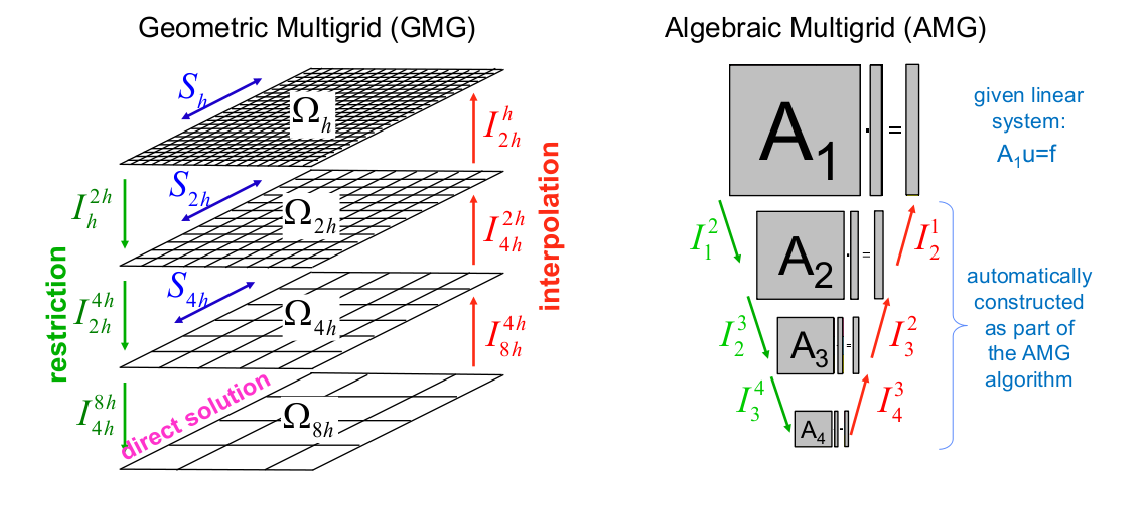
\includegraphics[width=1\textwidth]{chapters/ch03/GMGxAMG}
\caption{Comparison of Geometrical and Algebraic Multigrid approaches (from \cite{Trottenberg2001}).}
\label{fig:gmgxamg}
\end{figure}

Mathematically, both approaches can be described in almost the same way, it is just necessary to consider that meshes and nodes are linear system of equation and varibles of this system in AMG, respectively. Therefore, the Multigrid method can be briefly described for both approaches as follows:

Consider the system of equations on the finest level:
\begin{equation} \label{eq:mg1}
A_{f}p_{f} = f_{f}
\end{equation}
where $A_{f}$ is the matrix resultant from the procedure described in section \ref{sc:fem} and the subindex $f$ represent values on the fine level. After performing some iterations with a relaxation method, the error will be smoothed and its residual $r_{h}$ is:
\begin{equation} \label{eq:mg2}
A_{f}\hat{p_{f}} - f_{f} = r_{h}
\end{equation}
where $\hat{p_{f}}$ is the estimated solution for the variable of interest. Subtracting Eq. (\ref{eq:mg2}) from Eq. (\ref{eq:mg1}) yields:
\begin{equation} \label{eq:mg3}
A_{f}p_{f} - A_{f}\hat{p_{f}}= - r_{h}
\end{equation}
and if the operator $A_{h}$ is linear, this equation can be presented as a correction equation:
\begin{equation} \label{eq:mg4}
A_{f}\Delta p_{f}= - r_{h}
\end{equation}

Assuming, as already mentioned, that the high frequency modes of the error were already damped after the relaxation on the fine level, the reminiscent correction error will contain mainly low frequency modes and must be also solved, but in order to achieve this it is necessary to restrict it to a coarser level, where it will present itself as a high frequency mode, i.e.
\begin{equation} \label{eq:mg5}
A_{c}\Delta p_{c}= - I_{f}^{c}r_{f}
\end{equation}
In Eq. (\ref{eq:mg5}) $I_{f}^{c}$ represents the restriction operator, which transfer values from the residual in the fine level $f$ to the coarse level $c$. Once Eq. \ref{eq:mg5} is solved by means of an adequate solver (many times a direct solver will suffice, as this level presents lower storage and computation requirements), its solution can be interpolated back to the fine level using a prolongation operator $I_{c}^{f}$ and the original approximation on the fine level can then be corrected:
\begin{equation} \label{eq:mg6}
\hat{p_{f}^{\phantom{.}\ast}} = \hat{p_{f}} + I_{c}^{f} \Delta p_{c}
\end{equation}
where $\hat{p_{f}^{\phantom{.}\ast}}$ is the updated solution on the fine level. It is important to notice that this procedure is intrinsically recursive, so that the system on the coarse level could be seen as a new fine level, being itself smoothed again until some level is reached where the contributions of the corrections on the coarse levels are taken back to their respective fine levels. There are various schemes to handle this strategy, among them are the V-,W- and F-Cycle. Figure \ref{fig:mgcycles} shows a graphical representation of these cycles on a 4-level multigrid solution, see \cite{Briggs2000} or \cite{Trottenberg2001} for a detailed explanation of each of these cycles.

\begin{figure} 
\centering
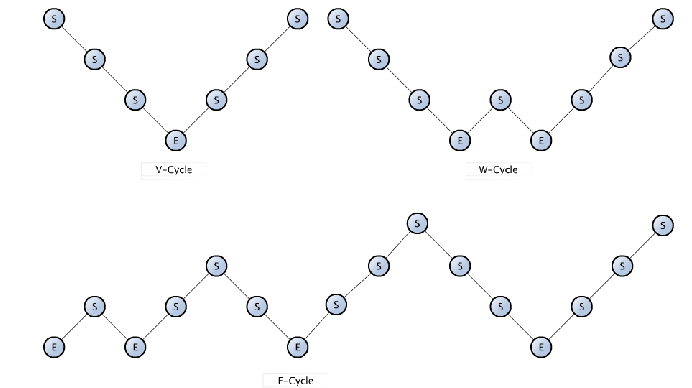
\includegraphics[width=0.9\textwidth]{chapters/ch03/MGCycles}
\caption{V- W- and F-Cycles. $S$ represents smoothing and $E$ is the solution on the coarsest level.}
\label{fig:mgcycles}
\end{figure}

